\documentclass{beamer}
\mode<presentation>
\usetheme{CambridgeUS}
\usepackage[russian]{babel}
\usepackage[utf8]{inputenc}
\usepackage[T2A]{fontenc}
\usepackage{sansmathaccent}
\pdfmapfile{+sansmathaccent.map}
\title{Пространственная обработка сигналов}
\author{Наумов Д.А.}
\date[08.04.2014] {Компьютерные музыкальные технологии и звуковой дизайн, 2014}

\begin{document}

%ТИТУЛЬНЫЙ СЛАЙД
\begin{frame}
  \titlepage
\end{frame}

%СОДЕРЖАНИЕ ЛЕКЦИИ
\begin{frame}
  \frametitle{Содержание лекции}
  \tableofcontents
\end{frame}

%РАЗДЕЛ 1
\section{Дилей}
\begin{frame}
  \textbf{Дилэй} (англ. \emph{delay}~--- задержка)~--- эффект задержки звука; задержка происходит с помощью записи входного сигнала с последующим проигрыванием его через определённый период времени. Задержанный сигнал может воспроизводится либо один раз, либо несколько раз для создания повторяющегося звука похожего на распадающейся эхо.

  \centering{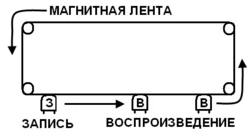
\includegraphics[width=0.5\textwidth]{pic-delay-01}}

  Первые эффекты дилэя создавались с помощью использования зацикленной магнитной ленты проигрываемой на магнитофоне.
\end{frame}

\begin{frame}
  Тонкая магнитная лента не совсем подходила для непрерывной работы, поэтому время от времени лента должна была заменяться для сохранения верности и качества задержанного звука.

  \begin{block}{Ленточный дилей Roland RE-201}
    \centering{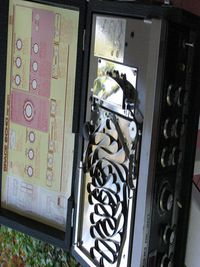
\includegraphics[width=0.25\textwidth]{pic-delay-02}}
  \end{block}
\end{frame}

\begin{frame}
  Другие популярные блоки как носитель использовали вращающийся магнитный барабан (к примеру дилэй \emph{Binson Echorec}. 
  
  \begin{block}{Дилэй Binson Echorec на основе магнитного барабана}
    \centering{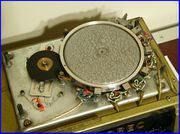
\includegraphics[width=0.3\textwidth]{pic-delay-03}}
  \end{block}
  
  Хотя аналоговые дилэи менее гибки чем цифровые и в целом имеют меньшее время задержки, несколько классических моделей, такие как \emph{Boss DM-2} по-прежнему ценятся за их "<теплое">, более естественное эхо. Кроме того, несколько компаний делают новые аналоговые дилэи, в их числе \emph{MXR Carbon Copy} и \emph{Ibanez AD9}, переиздавая свои педальные эффекты 1980-х годов.
\end{frame}

\begin{frame}
  Наличие недорогой цифровой обработки сигнала в конце 1970-х и 1980-х годов привело к разработке первых цифровых дилэев. Цифровые системы создавали задержку с помощью сэмплирования входного сигнала через аналого-цифровой преобразователь, после чего сигнал проходил через серию цифровых сигнальных процессоров, записывая сигнал в буфер хранения, а затем воспроизводя на основе установленных пользователем параметров.

  \begin{block}{Цифровой педальный дилэй Behringer Digital Delay DD400}
    \centering{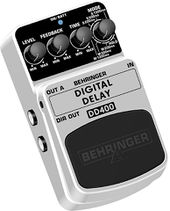
\includegraphics[width=0.25\textwidth]{pic-delay-04}}
  \end{block}
\end{frame}

\begin{frame}
  Многие современные цифровые дилэи имеют обширный набор вариантов настроек, включая:
  \begin{itemize}
    \item контроль времени до воспроизведения задержек сигнала (\emph{delay time});
    \item общий уровень обработанного сигнала по отношению к не обработанному (\emph{dry/wet});
    \item уровень на котором задержанный сигнал подается обратно в буфер, который будет снова повторяться ~--- так называемая \textbf{обратная связь} (\emph{feedback}).
  \end{itemize}  
  
  Программные дилэи во многих случаях предлагают гораздо большую гибкость, чем даже самые лучшие цифровое оборудование. Большое количество системной памяти современных персональных компьютеров предлагает практически безграничный буфер для хранения звука, и более натуральные алгоритмы задержки, предлагая возможность смещения или внесения случайности в задержки, или вставку других звуковых эффектов в процесс обратной связи.
\end{frame}

\begin{frame}
  Команда \emph{Effects > Delay and Echo > Delay} открывает диалоговое окно эффекта \emph{Delay}.
  
  \begin{block}{Окно эффекта \emph{Delay} в \emph{Adobe Audition}}
    \centering{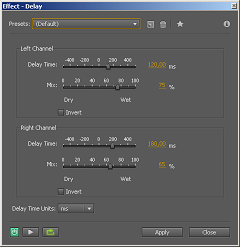
\includegraphics[width=0.5\textwidth]{pic-audelay-01}}
  \end{block}
\end{frame}

\begin{frame}
  Команда \emph{Effects > Delay and Echo > Analog Delay} открывает диалоговое окно эффекта, моделирует звучание устаревших аппаратных дилеев.

  \begin{block}{Окно эффекта \emph{Analog Delay} в \emph{Adobe Audition}}
    \centering{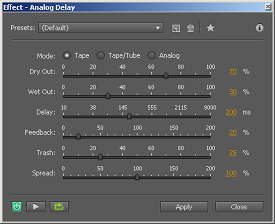
\includegraphics[width=0.5\textwidth]{pic-audelay-02}}
  \end{block}
\end{frame}

\begin{frame}
  В пакет \emph{Waves Platinum Native Bundle 4} входят два плагина, в которых реализованы многоотводные линии задержки:
  \begin{itemize}
    \item \emph{SuperTap 2~--- Taps Mode} является двухотводной линией задержки;
    \item \emph{SuperTap 6~--- Taps Mode} является шестиотводной линией задержки.
  \end{itemize}

  Возможна установка времени задержки в миллисекундах или согласование задержки с темпом композиции, ручной ввод темпа или ритма повторений, модуляция времени задержки посредством низкочастотного генератора, панорамирование и эквализация сигнала каждого отвода по отдельности.

  \centering{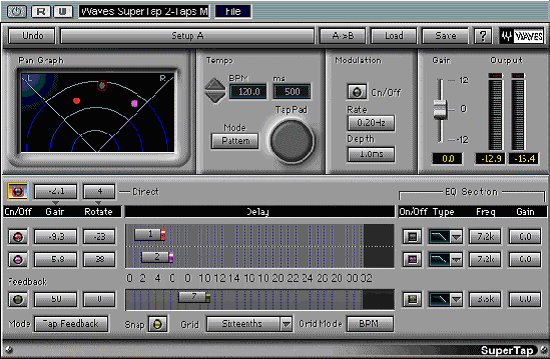
\includegraphics[width=0.5\textwidth]{pic-wavesdelay-01}}
  
\end{frame}

\section{Эхо}
\begin{frame}
  \textbf{Эхо} (англ. \emph{echo})~--- отражение звука, прибывающее к слушателю через некоторое время после прямого звука.

  ~

  В природе эхо образуется в результате отражения звуковых волн от препятствий (домов, стен помещения, гор и т. п.). Различные спектральные составляющие звука по-разному отражаются от препятствий: 
  
  \begin{itemize}
    \item Чем ниже частота, тем легче волна преодолевает препятствия.
    \item Высокочастотная волна не проходит сквозь препятствие, а отражается от него и частично поглощается. 
    \item Высокочастотные звуковые волны при распространении в воздухе затухают быстрее низкочастотных.
  \end{itemize} 

  ~

  Основное отличие \textbf{эффекта эхо} от эффекта дилей состоит в том, что задержанные копии сигнала подвергаются дополнительной обработке~--- изменяется их спектр. 
\end{frame}

\begin{frame}
С помощью диалогового окна эффекта \emph{Effects > Delay and Echo > Echo} можно смоделировать описанные ранее условия.

~
  
\centering{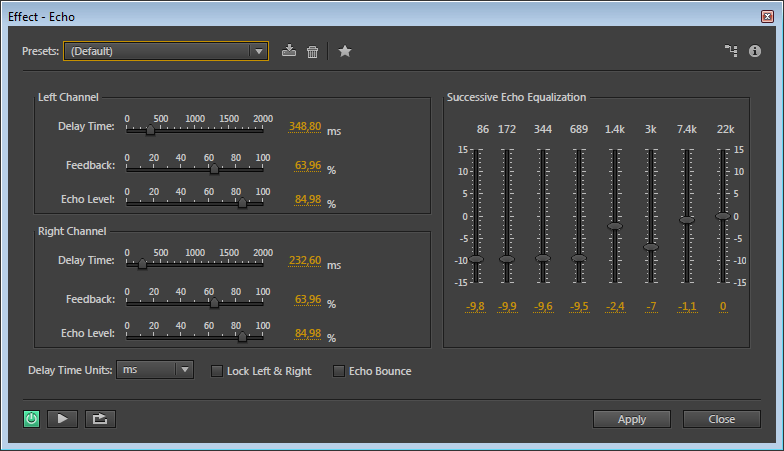
\includegraphics[width=0.75\textwidth]{pic-auecho-01}}

\end{frame}

\section{Реверберация}
\subsection{Распространение звука в замкнутом пространстве}
\begin{frame}
  Распространение звуковых волн в замкнутом пространстве отличается от распространения звука в открытом пространстве. Попадая на поверхность, звуковая волна:
  \begin{itemize}
    \item частично отражается от поверхности;
    \item частично поглощается материалом поверхности, переходя в тепловую энергию;
    \item незначительная ее доля проходит в соседнее помещение или пространство.
  \end{itemize}

  Какая именно часть энергии отражается обратно в помещение, определяет \textbf{коэффициент отражения} поверхности. Степень поглощения определяет \textbf{коэффициент поглощения}. Относительная мощность волны, прошедшей сквозь поверхность, задает \textbf{коэффициент звукопроводности}.
\end{frame}

\begin{frame}
  \begin{block}{Распространение звука в замкнутом пространстве}
    \centering{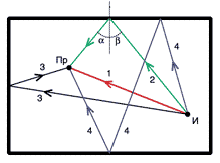
\includegraphics[width=0.5\textwidth]{pic-acoustic-01}}
  \end{block}
\end{frame}

\begin{frame}
  \begin{block}{Рефлектограмма идеального помещения}
    \centering{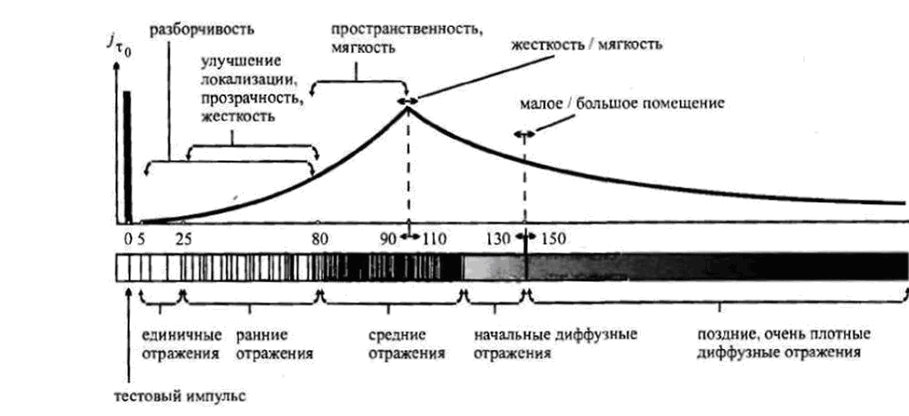
\includegraphics[width=0.75\textwidth]{pic-acoustic-02}}
  \end{block}
  
  ~
  
  $RT_{60}$ (\emph{Reverb time})~--- \textbf{время реверберации},~--- время, необходимое для того, чтобы отражения звука уменьшились на 60 дБ ниже уровня прямого звука.  
\end{frame}

\subsection{Особенности восприятия пространства}
\begin{frame}
  При определении направления и расстояния до источника звука используются следующие факторы:
  \begin{itemize}
    \item амплитуда: чем громче звук, тем ближе его источник.
    \item время: звук источника, расположенного слева, достигает левого уха на несколько микросекунд раньше, чем правого. 
    \item тембр: звуки, раздающиеся издалека, содержат меньше высоких частот. Воздействие тембра на направление сложнее~--- пока звук доходит от одного уха до другого, его тембр изменяется костями черепа и ушными раковинами. Попытка имитации этого эффекта называется \emph{head-related transfer function} (\emph{HRTF}).
    \item отражения от ближайших поверхностей (реверберация).
  \end{itemize}
\end{frame}

\begin{frame}
  Самыми важными при этом являются \textbf{ранние отражения}. В обычной прямоугольной комнате бывает от шести (пол, потолок и четыре стены) до десяти ранних отражений, прежде чем отражения начинают приходить столь часто, что сливаются в единую реверберацию.
  
  ~
  
 Ранние отражения воспринимаются нами не как повторения звука, а как информация об акустике помещения. Эта способность человеческого слуха называется "<\emph{эффект Хааса}">:
 
 \emph{если схожие звуки поступают с разных направлений с разницей по времени не более 50 миллисекунд, то мозг воспринимает только первый, более ранний звук, как отдельный, даже если последующие звуки громче первого на 10 дБ.}
 
 ~
 
 Наш мозг автоматически объединяет прямой звук и его повторения, в результате мы слышим один звук, но обогащенный информацией об акустике помещения.
\end{frame}

\begin{frame}
  Если просто объединить прямой звук и его задержанную копию, то произойдет изменение тембра звука, известное как результат действия "<гребенчатого фильтра">, то есть в определенном порядке одни частоты будут усилены, а другие ослаблены. Например, при объединении звука и его копии, задержанной на одну миллисекунду, будут усилены частоты 1 кГц, 2 кГц, 3 кГц и т. д., и ослаблены частоты 500 Гц, 1,5 кГц, 2,5 кГц и т. д. 

  \begin{block}{Изменения тембра при наложении звука и его задержанной во времени копии}
    \centering{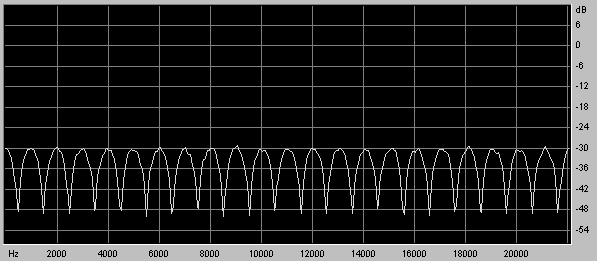
\includegraphics[width=0.75\textwidth]{pic-rever-02}}
  \end{block}  
\end{frame}

\subsection{Применение реверберации}
\begin{frame}
  \textbf{Ревербератор} (англ. \emph{reverberator})~--- устройство или программа, имитирующая эффект реверберации. Реверберация, созданная с помощью таких устройств, называется искусственной, и может выполнять следующие задачи:

  \begin{itemize}
    \item создание естественного пространственного эффекта;
    \item создание искусственных эффектов, которые не существуют в природе.
  \end{itemize}

  При создании эффекта сигнал изменяется так, что слушатель думает, что звук звучит в определенном пространстве (атмосфере), а не в "<сухой"> студии звукозаписи.
\end{frame}

\begin{frame}
  Первые эффекты реверберации создавались при помощи реального физического помещения, так называемых \textbf{эхо-камер}. В одном конце комнаты устанавливалась колонка, проигрывающая звук, а в другом микрофон, записывающий этот звук вместе с эффектом реверберации. Эта техника по прежнему используется, но она требует специальной звукоизоляции комнаты и создаёт одну из главных проблем~--- это трудность изменения времени реверберации.

  \begin{block}{Эхо-камера}
    \centering{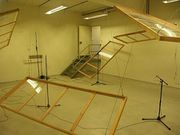
\includegraphics[width=0.5\textwidth]{pic-echochamber-01}}
  \end{block}  
\end{frame}

\begin{frame}
  \textbf{Цифровые ревербераторы} для создания эффекта реверберации используют различные математические алгоритмы. Вследствие того, что реверберация вызвана очень большим количеством эхо, простые алгоритмы ревербераторов используют несколько схем задержек и обратной связи для создания больших, распадающихся серий эхо.
  
  ~
  
  \textbf{Свёрточный (импульсный) ревербератор}~--- это цифровой процессор, моделирующий реверберацию физического или виртуального пространства на основе математической свёртки. В качестве свёртки используется предварительно записанный аудио сэмпл импульсного отклика моделируемого пространства. Процесс свёртки умножает каждый сэмпл звука для обработки (отражений) с сэмплами импульсного файла.  
\end{frame}

\begin{frame}
  \begin{block}{Пример импульсной характеристики помещения}
    \centering{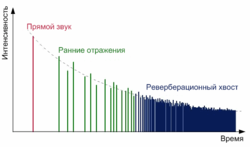
\includegraphics[width=0.75\textwidth]{pic-echochamber-02}}
  \end{block}
\end{frame}

\subsection{Эффекты реверберации в Adobe Audition}
\begin{frame}
  В \emph{Adobe Audition} реализованы следующие эффекты реверберации:
  \begin{itemize}
    \item \emph{Convolution Reverb}~--- позволяет создавать эффект реверберации на основе моделирования помещения с заданными характеристиками.
    \item \emph{Full Reverb}~--- эффект для моделирования реверберации с учетом размеров помещения, изменения спектра отраженно-го сигнала и т.д.
    \item \emph{Reverb}~--- позволяет моделировать реверберацию, но с меньшим количестом настроек, чем Full Reverb.
    \item \emph{Studio Reverb}~--- эффект для создания реверберации без моделирования помещения, за счет чего эффект получается менее требовательным к ресурсам процессора.
    \item \emph{Surround Reverb}~--- эффект для создания реверберации для звука в формате стерео 5.1.
  \end{itemize}  
\end{frame}

\begin{frame}
  \begin{block}{Окно эффекта Full Reverb, закладка Reverb Settings}
    \centering{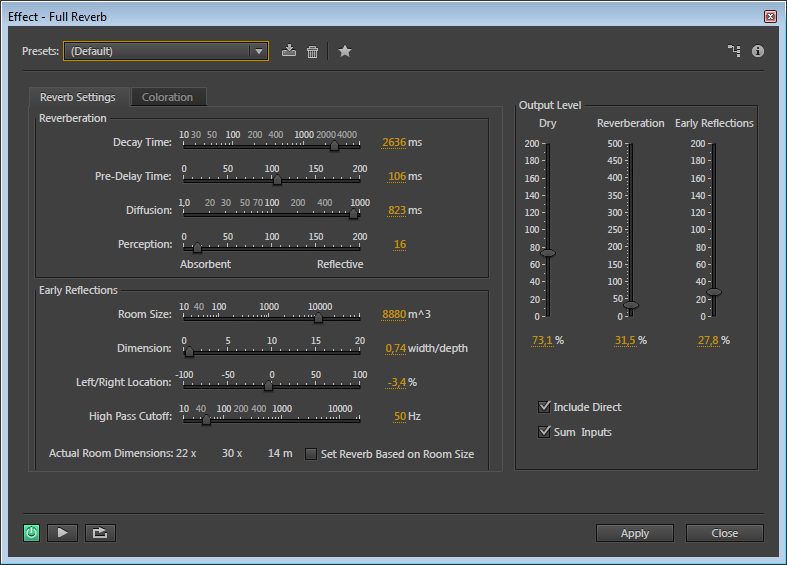
\includegraphics[width=0.75\textwidth]{pic-aureverb-01}}
  \end{block}
\end{frame}

\begin{frame}
  \begin{block}{Окно эффекта Full Reverb, закладка Coloration}
    \centering{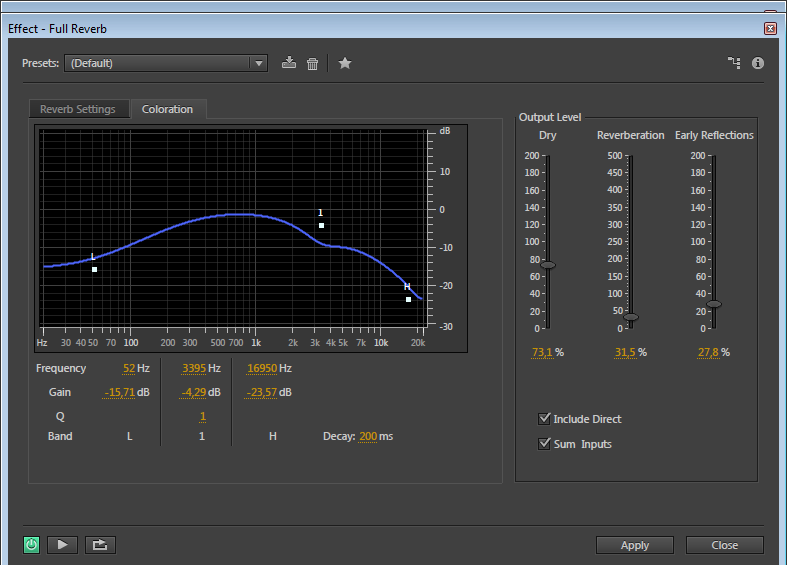
\includegraphics[width=0.75\textwidth]{pic-aureverb-02}}
  \end{block}
\end{frame}

\subsection{Эффекты реверберации пакета Waves}
\begin{frame}
  Эффект \emph{TrueVerb} создает реверберацию за счёт комбинации прямого звука, ранних отражений и реверберации.

  \begin{block}{Окно эффекта True Verb}
    \centering{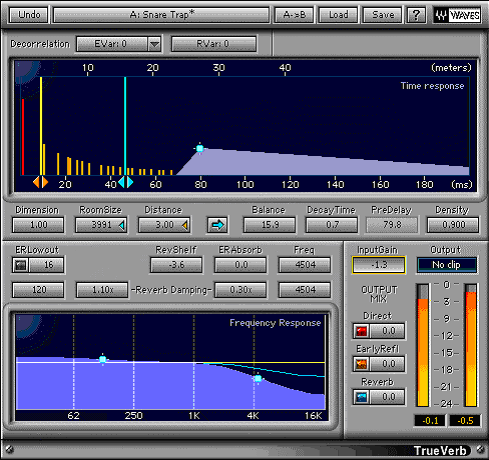
\includegraphics[width=0.6\textwidth]{pic-wavestrueverb-01}}
  \end{block}
\end{frame}

\begin{frame}
  Плагин \emph{RVerb} по своим возможностям подобен плагину \emph{TrueVerb}. Отличия заключаются в том, что характеристики входного и выходного фильтров ревербератора отображаются на различных дисплеях, кроме того, многие регуляторы выполнены в виде привычных и интуитивно понятных слайдеров.

  ~

  \begin{block}{Окно эффекта RVerb}
    \centering{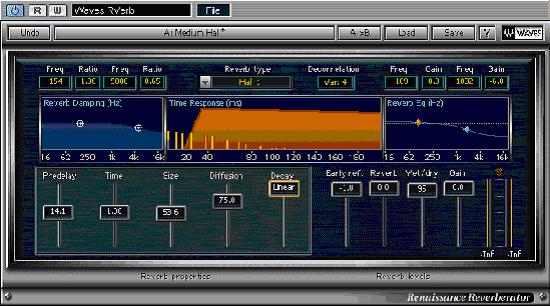
\includegraphics[width=0.75\textwidth]{pic-wavesrverb-01}}
  \end{block}
\end{frame}

\section{Применение эффектов дилей, эхо и реверберации}
\begin{frame}
  Запись \emph{track01} содержит примеры применения эффекта \emph{Analog Delay} в режимах \emph{Tape}, \emph{Tube} и \emph{Analog}.

  ~

  Запись \emph{track02} содержит примеры применения эффекта \emph{Echo}.

  ~

  Запись \emph{track03} содержит примеры применения эффекта реверберации:
  \begin{itemize}
    \item Часть 1 содержит два голоса, снятых на близкий микрофон в заглушённой студии.
    \item Часть 2 немного отличается: плотная реверберация имитирует большое, но поглощающее помещение, с близкими к камере голосами. Для большого и поглощающего помещения в части 2 ранние отражения начались в 40мсек и сгруппировались между 40 мсек и 100 мсек. Реверберационный хвост нарастает быстро, имеет широкую полосу и затухает через 0,3 секунды, микс был установлен на 40 процентов.
  \end{itemize}
\end{frame}  
          
\begin{frame}          
  \begin{itemize}
    \item Часть 3 соответствует меньшему помещению, но с более сильной реверберацией. Ранние отражения находятся между 16 мсек и 40 мсек. Реверберационный хвост также нарастает быстро и имеет около 0,7 секунды затухания, хотя высокие частоты затухают немного быстрее. Так как эта реверберация длиннее, то микс отчасти меньше: с использованием тех же настроек, что и в части 2, он был равен 25 процентам.
    \item Реверберационный хвост средней длины может помочь монтажным участкам музыки, позволяя инструментам затухать естественным образом через монтажный стык. Такая реверберация представлена в части 4. Вы, возможно, даже не заметите ее, когда играет музыка, но можете услышать ее в двух местах, когда музыка внезапно останавливается. Ранние отражения находятся в первых 50 мсек, затем реверберационный хвост очень быстро нарастает и имеет 3,3 секунды затухания. Микс равен 35 процентам.
  \end{itemize}
\end{frame}  

\begin{frame}
  \begin{itemize}
    \item В части 5 находятся голоса, звучащие внутри большого стального бака. Здесь нет ранних отражений, а реверберационный хвост начинается со средней скоростью атаки через несколько миллисекунд после прямого звука. Но хотя высокие частоты затухают примерно через две секунды, низким частотам для этого необходимо около 10 секунд.
    \item Вы можете добавить предварительную задержку для имитации огромного пространства. В результате получилась довольно хорошая железнодорожная система громкого оповещения, приведенная в части 6.
    \item Добавьте ФВЧ примерно на 500 Гц, чтобы имитировать потери в сети передачи сообщений, и она будет близкой к совершенству (часть 7).
  \end{itemize}
\end{frame}  

\end{document}
